\documentclass[aspectratio=169,11pt]{beamer}
\usepackage[utf8]{inputenc}
\usepackage[T1]{fontenc}
\usepackage[english]{babel}
\usepackage{amsmath,amssymb,booktabs,graphicx}
\usepackage{lmodern}

\definecolor{navy}{HTML}{183153}
\definecolor{teal}{HTML}{2A9D8F}
\definecolor{coral}{HTML}{D1495B}
\definecolor{sand}{HTML}{F4EDE4}
\setbeamercolor{structure}{fg=navy}
\setbeamercolor{frametitle}{fg=navy}
\setbeamercolor{title}{fg=navy}
\setbeamercolor{alerted text}{fg=coral}
\setbeamercolor{block title}{bg=navy,fg=white}
\setbeamercolor{block body}{bg=sand,fg=black}
\setbeamertemplate{navigation symbols}{}
\setbeamertemplate{footline}[frame number]
\setbeamerfont{frametitle}{size=\Large,series=\bfseries}
\setbeamerfont{title}{size=\Huge,series=\bfseries}

% Verified repository URL; the visible label is shortened for readability.
\newcommand{\RepoURL}{https://github.com/alejandroventuraventurameza-tech/ai-02-agrawal}
\newcommand{\sourcefoot}{%
  \vfill\hfill\scriptsize\color{gray}
  Source: Agrawal, Gans \& Goldfarb (2025), NBER WP 34034.}

\title{The Economics of Bicycles for the Mind}
\subtitle{What AI substitutes, what it amplifies, and the variance trap}
\author{Repository 2 analysis}
\date{AI \& Economic Modeling \textperiodcentered{} Week of August 24--29}

\begin{document}

%================= TITLE ==============================================
\begin{frame}[plain]
  \titlepage
  \begin{center}\small\color{teal}
    \href{\RepoURL}{\texttt{github.com/alejandroventuraventurameza-tech/ai-02-agrawal}}
  \end{center}
\end{frame}

%================= 1. PAPER ===========================================
\begin{frame}{1 \textperiodcentered{} A tool replaces execution but amplifies judgment}
  \textbf{Question.} When a cognitive tool makes implementation easier, how do
  effort, productivity, and inequality change?

  \medskip
  \begin{columns}[T,onlytextwidth]
    \column{0.43\textwidth}
    \textbf{Three human capabilities}
    \begin{itemize}\small
      \item $s$: implementation skill
      \item $\alpha$: payoff judgment
      \item $(\gamma_0,\gamma)$: opportunity judgment
    \end{itemize}

    \column{0.53\textwidth}
    \textbf{The agent's problem}
    \[
      \max_{e\ge0}\;
      \underbrace{p(se;\theta)\alpha\Delta}_{\text{expected improvement}}
      -\underbrace{c(e;\theta)}_{\text{effort cost}}
    \]
    \[
      V(\theta)=
      \underbrace{\frac{\gamma_0}{1-\delta\gamma}}_{\Gamma:
      \text{ opportunity multiplier}}M(e^*(\theta);\theta)
    \]
  \end{columns}

  \begin{block}{Single mechanism}
    The tool lowers the return to extra human implementation effort, while
    better opportunity judgment multiplies every gain the tool creates.
  \end{block}
  \sourcefoot
\end{frame}

%================= 2. MAIN RESULT =====================================
\begin{frame}{2 \textperiodcentered{} Proposition 3 is conditional, not a slogan}
  \small
  \textbf{Additional assumptions:}
  $p(se;\theta)=\sqrt{se+\theta}$, $c(e)=e$; mutually independent positive
  $(\alpha,\gamma_0,\gamma,s)$; $\delta\gamma<1$; and an interior optimum.

  \[
    V(\theta)=\Gamma\left(\frac{\alpha^2\Delta^2s}{4}+\frac{\theta}{s}\right),
    \qquad \Gamma=\frac{\gamma_0}{1-\delta\gamma}.
  \]

  \begin{columns}[T,onlytextwidth]
    \column{0.47\textwidth}
    \textbf{Heterogeneity threshold}
    \[
      \frac{E[\Gamma^2]}{E[\Gamma]^2}<E[s]E[1/s].
    \]
    It makes the initial variance slope negative.

    \column{0.49\textwidth}
    \textbf{Exact derivative}
    \[
      \frac{d\operatorname{Var}(V)}{d\theta}
      =a_0+2\theta\operatorname{Var}(\Gamma/s).
    \]
    It turns at $\theta^*=-a_0/[2\operatorname{Var}(\Gamma/s)]$.
  \end{columns}

  \begin{alertblock}{Condition missing from the published statement}
    A positive slope at $\theta=1$ additionally requires $\theta^*<1$.
    The threshold above proves only $\theta^*>0$.
  \end{alertblock}
  \sourcefoot
\end{frame}

%================= 3. WHAT I DID ======================================
\begin{frame}{3 \textperiodcentered{} Capping the probability removes the U in this example}
  \begin{columns}[T,onlytextwidth]
    \column{0.60\textwidth}
    \IfFileExists{figures/prop3-bounded-success.png}{
      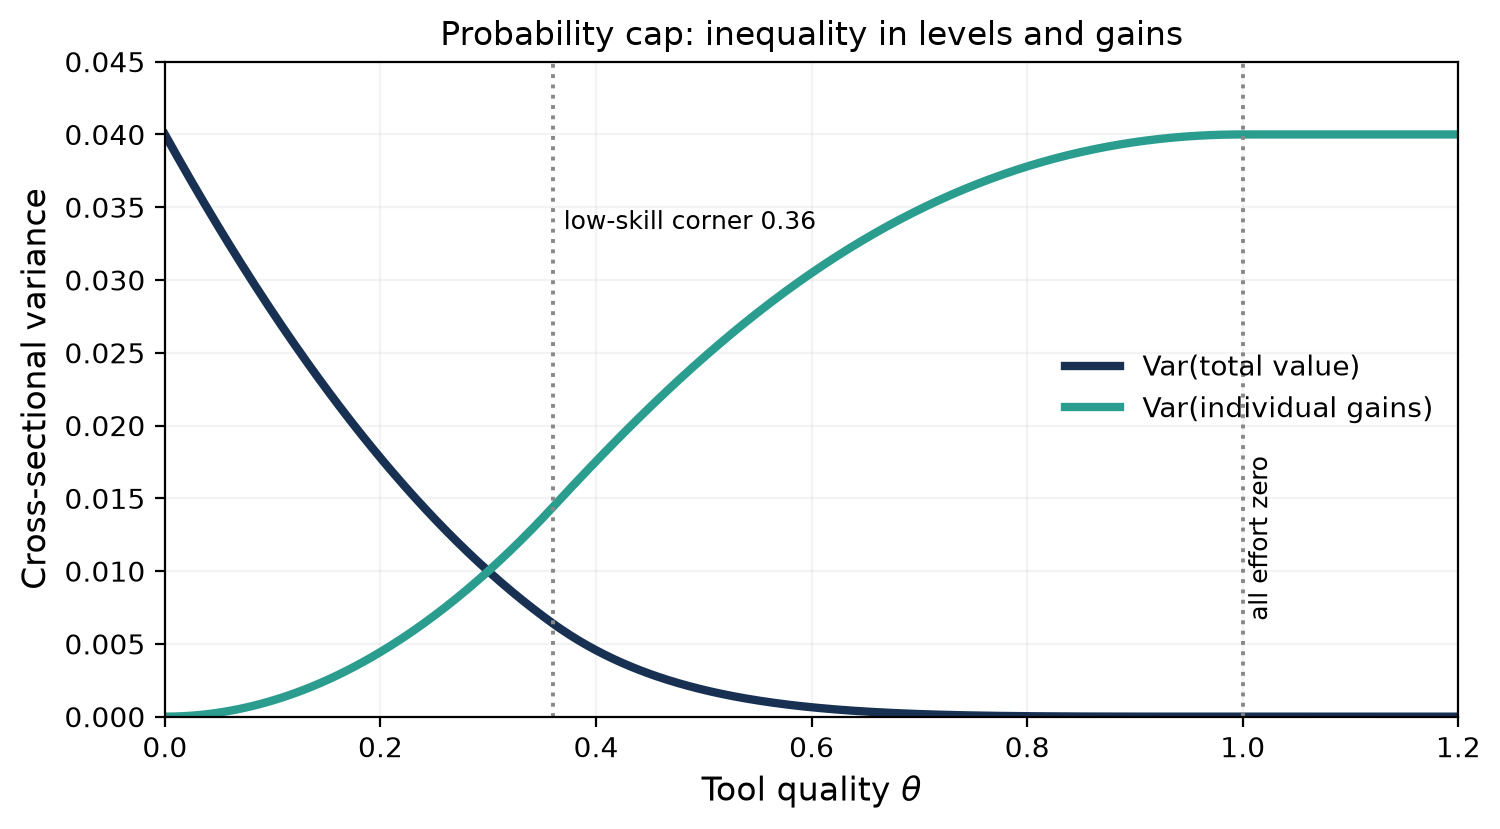
\includegraphics[width=\linewidth]{figures/prop3-bounded-success.png}
    }{
      \fbox{\parbox[c][0.48\textheight][c]{0.95\linewidth}{\centering
        Run \texttt{python bounded_model.py} to generate the figure.}}
    }

    \column{0.36\textwidth}
    \textbf{My separate extension}
    \begin{itemize}\small
      \item $p=\min\{1,\sqrt{se+\theta}\}$
      \item $\Gamma=\alpha=1$, $\Delta=2$
      \item $s\in\{0.6,1\}$, equally likely
      \item Level variance $\downarrow 0$
      \item Gain variance $\uparrow 0.04$
    \end{itemize}

    \textbf{Why?}
    {\small Low-skill effort hits zero at
    $\theta=0.36$; all effort is zero by $\theta=1$.}

    \medskip
    {\scriptsize\color{gray}Own model variant; the cap changes the
    global strict-substitution assumption.}
  \end{columns}
  \sourcefoot
\end{frame}

%================= 4. AI CHECK ========================================
\begin{frame}{4 \textperiodcentered{} I checked the AI's example, not just its algebra}
  \begin{columns}[T,onlytextwidth]
    \column{0.47\textwidth}
    \textbf{The recorded AI answer}
    {\small Claimed an admissible counterexample after
    checking (H) and interiority (see \texttt{prompts.md}).}

    \medskip
    \textbf{Three independent checks}
    \begin{itemize}\small
      \item (H) holds, yet $\operatorname{Var}'(1)=-14/45$.
      A reversal at 1 needs $\theta^*<1$.
      \item $p^*=2s\in\{1.2,2\}>1$:
      not a probability.
      \item The corner $1.44$ comes before the
      algebraic turn $2.4$.
    \end{itemize}

    \begin{alertblock}{Verdict}
      \small\textbf{Incorrect as a probability model};
      its algebra is valid, but its calibration is not.
    \end{alertblock}

    \column{0.49\textwidth}
    \textbf{Handwritten audit (page 4 of 4)}

    \IfFileExists{hand/prop3-derivation.jpg}{
      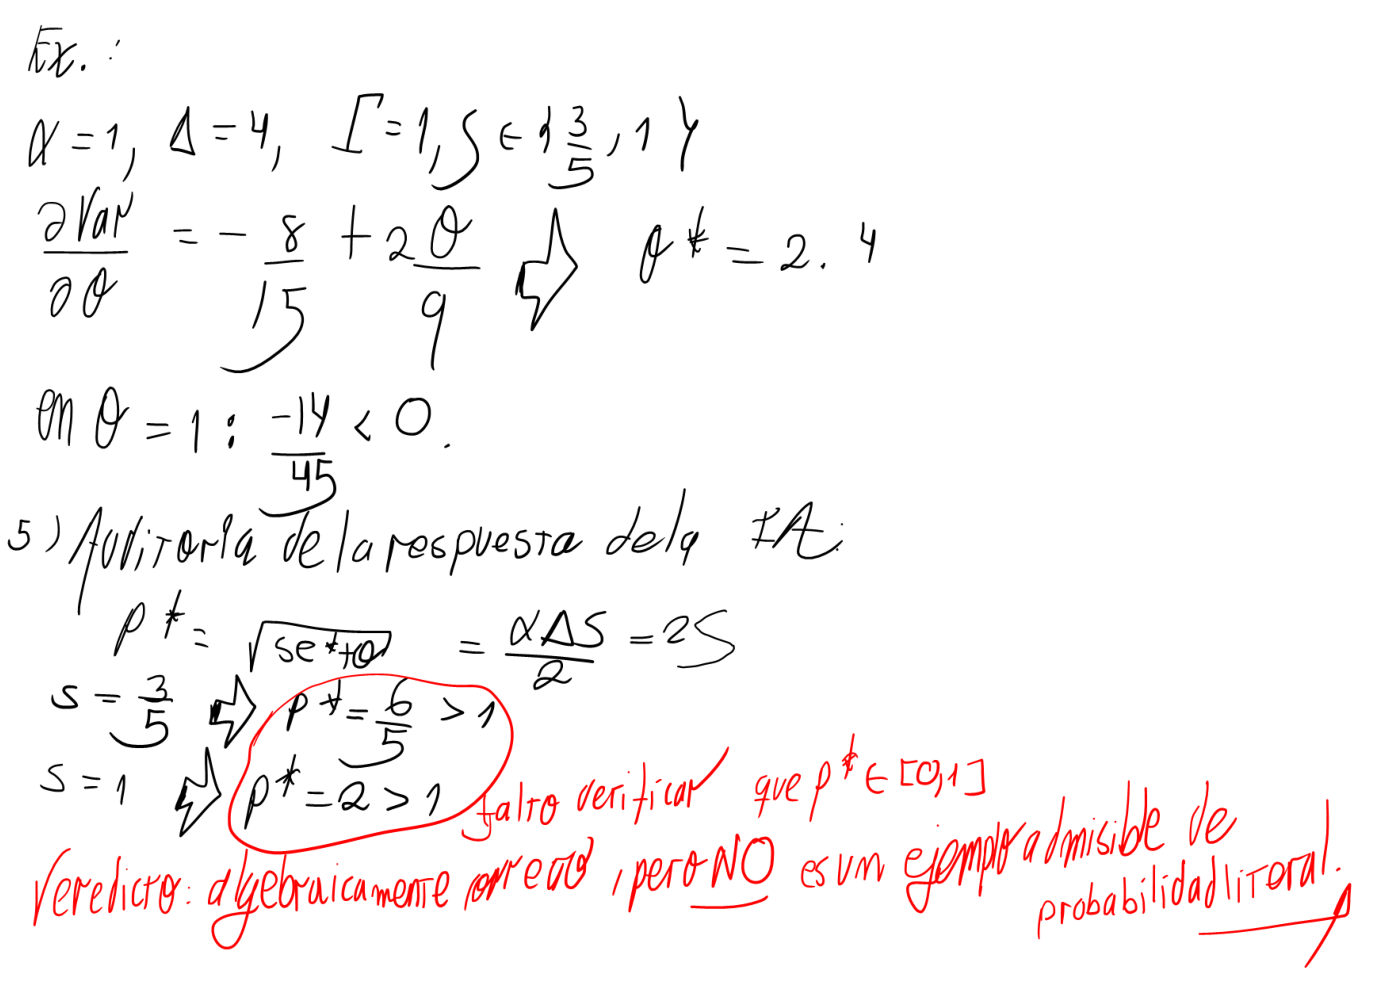
\includegraphics[width=\linewidth,height=0.59\textheight,keepaspectratio]
      {hand/prop3-derivation.jpg}

      {\scriptsize\color{gray}Original full derivation: \texttt{hand/prop3-handwritten-full.pdf}}
    }{
      \IfFileExists{hand/prop3-derivation.png}{
        \includegraphics[width=\linewidth,height=0.53\textheight,keepaspectratio]
        {hand/prop3-derivation.png}
      }{
        \fbox{\parbox[c][0.45\textheight][c]{0.92\linewidth}{\centering
          \textbf{Add the real phone photo here}\\[0.7em]
          \texttt{hand/prop3-derivation.jpg}\\[0.7em]
          FOC $\to e^*$ $\to$ interior condition $\to$ variance derivative.}}
      }
    }
  \end{columns}
  \sourcefoot
\end{frame}

\end{document}
